% Options for packages loaded elsewhere
\PassOptionsToPackage{unicode}{hyperref}
\PassOptionsToPackage{hyphens}{url}
\PassOptionsToPackage{dvipsnames,svgnames,x11names}{xcolor}
%
\documentclass[
  authoryear,
  review,
  3p]{elsarticle}

\usepackage{amsmath,amssymb}
\usepackage{iftex}
\ifPDFTeX
  \usepackage[T1]{fontenc}
  \usepackage[utf8]{inputenc}
  \usepackage{textcomp} % provide euro and other symbols
\else % if luatex or xetex
  \usepackage{unicode-math}
  \defaultfontfeatures{Scale=MatchLowercase}
  \defaultfontfeatures[\rmfamily]{Ligatures=TeX,Scale=1}
\fi
\usepackage{lmodern}
\ifPDFTeX\else  
    % xetex/luatex font selection
\fi
% Use upquote if available, for straight quotes in verbatim environments
\IfFileExists{upquote.sty}{\usepackage{upquote}}{}
\IfFileExists{microtype.sty}{% use microtype if available
  \usepackage[]{microtype}
  \UseMicrotypeSet[protrusion]{basicmath} % disable protrusion for tt fonts
}{}
\makeatletter
\@ifundefined{KOMAClassName}{% if non-KOMA class
  \IfFileExists{parskip.sty}{%
    \usepackage{parskip}
  }{% else
    \setlength{\parindent}{0pt}
    \setlength{\parskip}{6pt plus 2pt minus 1pt}}
}{% if KOMA class
  \KOMAoptions{parskip=half}}
\makeatother
\usepackage{xcolor}
\setlength{\emergencystretch}{3em} % prevent overfull lines
\setcounter{secnumdepth}{5}
% Make \paragraph and \subparagraph free-standing
\ifx\paragraph\undefined\else
  \let\oldparagraph\paragraph
  \renewcommand{\paragraph}[1]{\oldparagraph{#1}\mbox{}}
\fi
\ifx\subparagraph\undefined\else
  \let\oldsubparagraph\subparagraph
  \renewcommand{\subparagraph}[1]{\oldsubparagraph{#1}\mbox{}}
\fi


\providecommand{\tightlist}{%
  \setlength{\itemsep}{0pt}\setlength{\parskip}{0pt}}\usepackage{longtable,booktabs,array}
\usepackage{calc} % for calculating minipage widths
% Correct order of tables after \paragraph or \subparagraph
\usepackage{etoolbox}
\makeatletter
\patchcmd\longtable{\par}{\if@noskipsec\mbox{}\fi\par}{}{}
\makeatother
% Allow footnotes in longtable head/foot
\IfFileExists{footnotehyper.sty}{\usepackage{footnotehyper}}{\usepackage{footnote}}
\makesavenoteenv{longtable}
\usepackage{graphicx}
\makeatletter
\def\maxwidth{\ifdim\Gin@nat@width>\linewidth\linewidth\else\Gin@nat@width\fi}
\def\maxheight{\ifdim\Gin@nat@height>\textheight\textheight\else\Gin@nat@height\fi}
\makeatother
% Scale images if necessary, so that they will not overflow the page
% margins by default, and it is still possible to overwrite the defaults
% using explicit options in \includegraphics[width, height, ...]{}
\setkeys{Gin}{width=\maxwidth,height=\maxheight,keepaspectratio}
% Set default figure placement to htbp
\makeatletter
\def\fps@figure{htbp}
\makeatother

\newcommand{\mycommand}[1]{\textbf{#1}}
\makeatletter
\makeatother
\makeatletter
\makeatother
\makeatletter
\@ifpackageloaded{caption}{}{\usepackage{caption}}
\AtBeginDocument{%
\ifdefined\contentsname
  \renewcommand*\contentsname{Table of contents}
\else
  \newcommand\contentsname{Table of contents}
\fi
\ifdefined\listfigurename
  \renewcommand*\listfigurename{List of Figures}
\else
  \newcommand\listfigurename{List of Figures}
\fi
\ifdefined\listtablename
  \renewcommand*\listtablename{List of Tables}
\else
  \newcommand\listtablename{List of Tables}
\fi
\ifdefined\figurename
  \renewcommand*\figurename{Figure}
\else
  \newcommand\figurename{Figure}
\fi
\ifdefined\tablename
  \renewcommand*\tablename{Table}
\else
  \newcommand\tablename{Table}
\fi
}
\@ifpackageloaded{float}{}{\usepackage{float}}
\floatstyle{ruled}
\@ifundefined{c@chapter}{\newfloat{codelisting}{h}{lop}}{\newfloat{codelisting}{h}{lop}[chapter]}
\floatname{codelisting}{Listing}
\newcommand*\listoflistings{\listof{codelisting}{List of Listings}}
\makeatother
\makeatletter
\@ifpackageloaded{caption}{}{\usepackage{caption}}
\@ifpackageloaded{subcaption}{}{\usepackage{subcaption}}
\makeatother
\makeatletter
\@ifpackageloaded{tcolorbox}{}{\usepackage[skins,breakable]{tcolorbox}}
\makeatother
\makeatletter
\@ifundefined{shadecolor}{\definecolor{shadecolor}{rgb}{.97, .97, .97}}
\makeatother
\makeatletter
\makeatother
\makeatletter
\@ifpackageloaded{sidenotes}{}{\usepackage{sidenotes}}
\@ifpackageloaded{marginnote}{}{\usepackage{marginnote}}
\makeatother
\makeatletter
\makeatother
\journal{Journal of Animal Biotelemetry}
\ifLuaTeX
  \usepackage{selnolig}  % disable illegal ligatures
\fi
\usepackage[]{natbib}
\bibliographystyle{elsarticle-harv}
\IfFileExists{bookmark.sty}{\usepackage{bookmark}}{\usepackage{hyperref}}
\IfFileExists{xurl.sty}{\usepackage{xurl}}{} % add URL line breaks if available
\urlstyle{same} % disable monospaced font for URLs
\hypersetup{
  pdftitle={Vertical movement behaviour of the starry smooth-hound shark Mustelus asterias in the North Sea},
  pdfauthor={Lotte Pohl; Niels Brevé; Carlota Muñiz; Jan Reubens},
  pdfkeywords={acoustic telemetry, geolocation modelling, mustelus
asterias},
  colorlinks=true,
  linkcolor={blue},
  filecolor={Maroon},
  citecolor={Blue},
  urlcolor={Blue},
  pdfcreator={LaTeX via pandoc}}

\setlength{\parindent}{6pt}
\begin{document}

\begin{frontmatter}
\title{Vertical movement behaviour of the starry smooth-hound shark
\emph{Mustelus asterias} in the North Sea \\\large{Master Thesis} }
\author[1,2]{Lotte Pohl%
\corref{cor1}%
\fnref{fn1}}
 \ead{lotte.pohl@imbrsea.eu} 
\author[3,4]{Niels Brevé%
%
\fnref{fn2}}
 \ead{breve@sportvisserijnederland.nl} 
\author[1]{Carlota Muñiz%
%
\fnref{fn3}}
 \ead{carlota.muniz@vliz.be} 
\author[1]{Jan Reubens%
%
\fnref{fn4}}
 \ead{jan.reubens@vliz.be} 

\affiliation[1]{organization={Flemish Marine Institute, Marine
Observation Centre},addressline={Slipwaykaai
2},city={Ostend},postcode={8400},postcodesep={}}
\affiliation[2]{organization={Ghent University, Marine Biology research
group},addressline={Krijgslaan
281/S8},city={Ghent},postcode={9000},postcodesep={}}
\affiliation[3]{organization={Wageningen University and Research, Marine
Ecology Group},addressline={Droevendaalsesteeg
1},city={Wageningen},postcode={6700},postcodesep={}}
\affiliation[4]{organization={Sportvisserij
Nederlands},addressline={Leyenseweg
115},city={Bilthoven},postcode={3721},postcodesep={}}

\cortext[cor1]{Corresponding author}
\fntext[fn1]{Msc Student}
\fntext[fn2]{Second Promotor}
\fntext[fn3]{Supervisor}
\fntext[fn4]{Promotor}
        
\begin{abstract}
Still to be written.
\end{abstract}





\begin{keyword}
    acoustic telemetry \sep geolocation modelling \sep 
    mustelus asterias
\end{keyword}
\end{frontmatter}
    \ifdefined\Shaded\renewenvironment{Shaded}{\begin{tcolorbox}[frame hidden, breakable, enhanced, borderline west={3pt}{0pt}{shadecolor}, interior hidden, sharp corners, boxrule=0pt]}{\end{tcolorbox}}\fi

\renewcommand*\contentsname{Table of contents}
{
\hypersetup{linkcolor=}
\setcounter{tocdepth}{3}
\tableofcontents
}
\hypertarget{introduction}{%
\section{Introduction}\label{introduction}}

Here is some normal text, and then we'll use the
\mycommand{custom command} to make this text bold. Also, this is a
reference test \citet{dodge_2013}. And to combine references, we can use
this \citep{nathan_2008, dodge_2013}

\hypertarget{materials-and-methods}{%
\section{Materials and Methods}\label{materials-and-methods}}

\hypertarget{results}{%
\section{Results}\label{results}}

\hypertarget{data-storage-tags}{%
\subsection{Data Storage Tags}\label{data-storage-tags}}

The depth log of tag 304 is shown below (see Figure~\ref{fig-dst304}).

\begin{figure}

{\centering 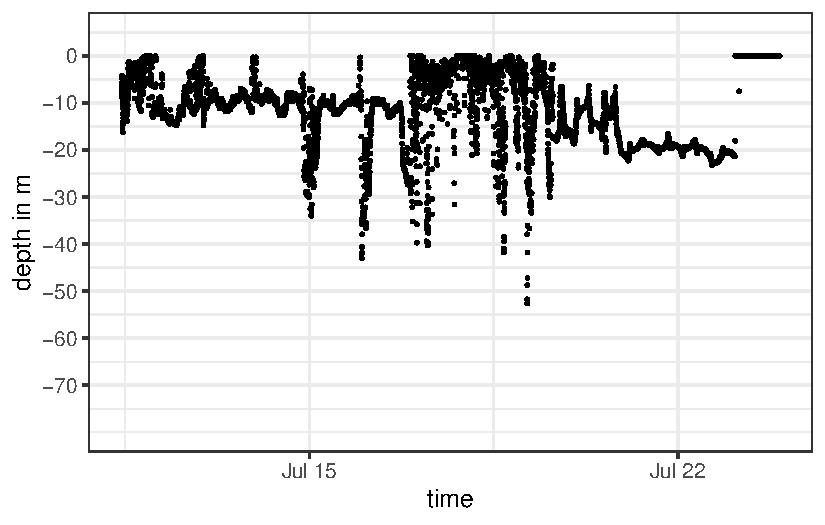
\includegraphics[width=0.5\textwidth,height=\textheight]{index_files/figure-pdf/fig-dst304-1.pdf}

}

\caption{\label{fig-dst304}Depth log from the recovered tag 304.}

\end{figure}

\hypertarget{summary-statistics}{%
\subsubsection{Summary statistics}\label{summary-statistics}}

Below the summary statistics for dst tag 308 are displayed
(Figure~\ref{fig-dstsummary308}).

\begin{figure}

\begin{minipage}[t]{0.50\linewidth}

{\centering 

\raisebox{-\height}{

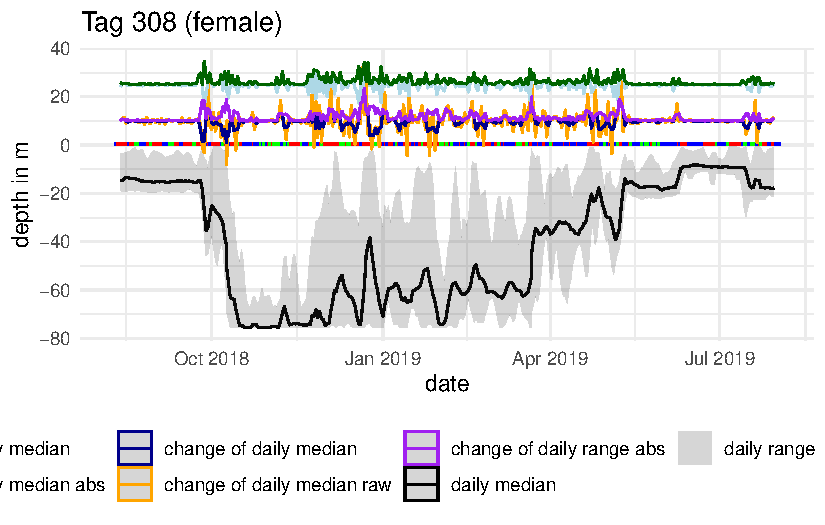
\includegraphics{index_files/figure-pdf/fig-dstsummary308-1.pdf}

}

}

\subcaption{\label{fig-dstsummary308-1}Daily median depth and depth
range of tag 308.}
\end{minipage}%
%
\begin{minipage}[t]{0.50\linewidth}

{\centering 

\raisebox{-\height}{

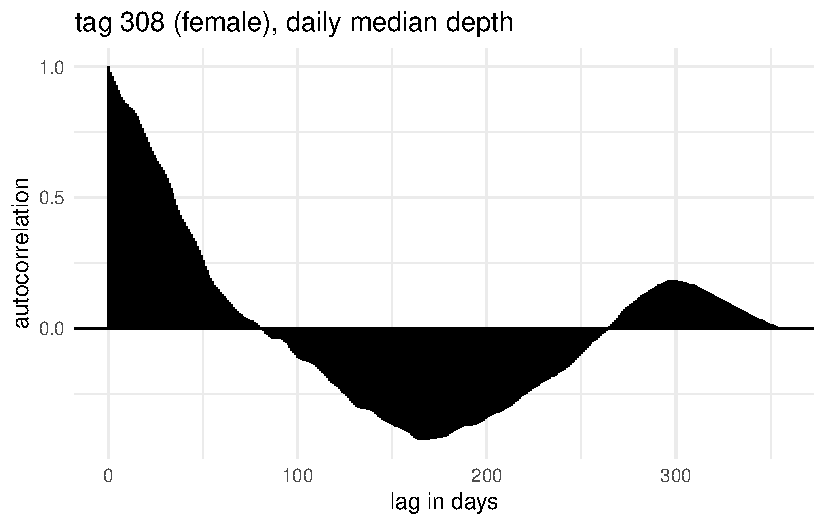
\includegraphics{index_files/figure-pdf/fig-dstsummary308-2.pdf}

}

}

\subcaption{\label{fig-dstsummary308-2}Autocorrelation of the daily
median depth.}
\end{minipage}%

\caption{\label{fig-dstsummary308}Summary statistics for tag 308.}

\end{figure}

\hypertarget{discussion}{%
\section{Discussion}\label{discussion}}


\renewcommand\refname{References}
  \bibliography{bibliography.bib}


\end{document}
